
\documentclass[a4paper]{article}
\usepackage[pdftex]{graphicx}
\usepackage[utf8]{inputenc}
\usepackage{enumerate}
\usepackage{siunitx}
\sisetup{locale=DE} 
\usepackage{icomma}
\usepackage{amssymb}
\usepackage{tikz}
\usepackage{href-ul}
\hypersetup{
	colorlinks=true,
	linkcolor=blue,
	urlcolor=blue}
\usepackage{geometry}
\geometry{a4paper, top=15mm, left=15mm, right=15mm, bottom=15mm,
	headsep=10mm, footskip=12mm}

\begin{document}
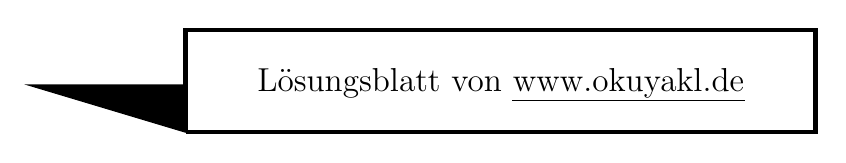
\begin{tikzpicture}(10,3)
	\draw[ultra thick](2,0) --(10,0) -- (10,1.3) --(2,1.3) -- (2,0);
	\draw[fill=black](2,0)-- (0,.6) -- (2,.6) -- (2,0);
	\node at (6,.6) {\large Lösungsblatt von \href{https://www.okuyakl.de}{www.okuyakl.de}};
\end{tikzpicture}
\vspace{0.5 cm}


\noindent {\bf Aufgabe 1.}\\
Während des Ladens baut sich im Kondensator eine Spannung auf, die der angelegten Spannung entgegen wirkt. Darum ist der Ladestrom zuerst groß und nimmt dann exponentiell ab.
\vspace{0.5 cm}

\noindent {\bf Aufgabe 2.}\\
Das Kügelchen wird von der positiv geladenen Platte des Kondensators angezogen. Auf seinem Weg dorthin legt es die Strecke $d/2$ zurück. Die wirkende Coulombkraft $F_C$ verrichtet die Arbeit 
$$W_{el} = F_C \cdot {d \over 2}$$ die wir mit der kinetischen Energie $E_{kin}$ des Kügelchens gleichsetzen und nach $v(d)$ auflösen:

$$
\renewcommand{\arraystretch}{2}
\begin{array}{rcll}
W_{el} & = & E_{kin} \\
F_C \cdot {d \over 2} & = & {1 \over 2}m v(d)^2 \\
q \cdot E \cdot {d \over 2} & = & {1 \over 2}m v(d)^2 & | \cdot 2 : m \\
{q \cdot E \cdot d \over m} & = & v(d)^2 & | \sqrt{\quad}\\
v(d) & = & \sqrt{q \cdot E \cdot d \over m} &|(*) \\
v(d) & = & \sqrt{q \cdot E \over m} \cdot \sqrt{d} \\
v(d) & = & \sqrt{\SI{1,4e-9}{\coulomb} \cdot \SI{36e3}{\volt\over \meter}\over \SI{12e-6}{\kilogram}}  \cdot \sqrt{d}\\ 
 & = & 2,0 \cdot \sqrt{\SI{}{\coulomb \cdot \volt \over \kilogram \cdot \meter}}  \cdot \sqrt{d} \\
 & = & 2,0 \cdot \sqrt{ \SI{}{\joule \over \kilogram \cdot \meter}}  \cdot \sqrt{d}\\
 & = & 2,0  \cdot \sqrt{\SI{}{{\kilogram \cdot \meter^2 \cdot \second^{-2}} \over {\kilogram \cdot \meter}}} \cdot \sqrt{d}\\
 & = & \SI{2,0}{\sqrt{\meter}\over \second} \cdot \sqrt{d}
\end{array}
$$
\vspace{0.5 cm}

\noindent {\bf Aufgabe 3.}\\
Es gilt für die Spannung:
$$ U = E \cdot d $$
Der Faktor $E \cdot d $ aus $(*)$ ersetzen wir also durch $U$:
$$ v = \sqrt{q \cdot U \over m} \quad (**)$$
Anschließend lösen wir nach der Spannung auf und setzen ein:
$$ 
\renewcommand{\arraystretch}{2}
\begin{array}{rcl}
U & = & {v^2 \cdot m \over q} \\
  & = & {(\SI{0,56}{\meter\over \second})^2 \cdot \SI{12e-6}{\kilogram} \over \SI{1,4e-9}{\coulomb}}\\
  & = & \SI{2688}{\volt}\\
  & = & \SI{2,7}{\kilo\volt}
\end{array}
$$
Einheitencheck:

$$\SI{}{\meter^2\cdot \second^{-2}\kilogram \over \coulomb}=\SI{}{\joule\over \coulomb}=\SI{}{\volt}$$
\vspace{0.5 cm}

\noindent {\bf Aufgabe 4.}\\
Der Plattenabstand $d$ kommt in der Formel $(**)$ nicht mehr vor;
bei bestehender Verbindung zur Spannungsquelle bleibt $U$ konstant, also ändert sich $v$ nicht.
\vspace{0.5 cm}

\noindent {\bf Aufgabe 5.}\\ 
Beim Kontakt mit der positiv geladenen Platte wird das Kügelchen ebenfalls positiv geladen und folglich abgestoßen. Nun wirkt die Coulombkraft in die andere Richtung und das Kügelchen bewegt sich  zur negativen Platte, wo es wieder umgeladen wird, die Richtung wechselt und so weiter...
  
 \begin{center}
 	\includegraphics[width=7 cm]{../../viecher/endcomic.pdf}
 	
 	Hier geht es zurück zum \href{https://www.okuyakl.de/phys/p12efeldL093/aa093.pdf}{Aufgabenblatt}
 \end{center}
 
\end{document}